\documentclass[11pt,a4paper]{article}
\usepackage[margin=2.15cm]{geometry}
\usepackage[T1]{fontenc}
\usepackage[utf8]{inputenc}
\usepackage{amsmath,amssymb,booktabs,longtable,tabularx,array,enumitem,microtype}
\usepackage{graphicx,float,xcolor}
\usepackage{hyperref}
\hypersetup{
  colorlinks=true,
  linkcolor=blue!55!black,
  urlcolor=blue!55!black,
  pdftitle={FIN Local Research Checkpoint P428--P430},
  pdfauthor={Krzysztof Żuchowski},
  pdfsubject={Type-correct cosine reduction, exact-rational Krawczyk certificate, and global dual feasibility},
  pdfkeywords={FIN, cosine, Lean, Krawczyk method, signed moments, Bernstein polynomial, Legacy kernel, mathematical physics}
}
\setlist{nosep,leftmargin=*}
\setlength{\parindent}{0pt}
\setlength{\parskip}{0.52em}
\renewcommand{\arraystretch}{1.16}
\newcommand{\status}[1]{\textbf{[#1]}}
\newcommand{\Klegacy}{K_{\mathrm{legacy,ont}}}
\newcommand{\Kstrict}{K_{\mathrm{strict,gate}}}
\newcommand{\Kstar}{K^*_{\mathrm{legacy}}}
\newcolumntype{Y}{>{\raggedright\arraybackslash}X}

\begin{document}

\begin{titlepage}
\centering
{\Large FIN Local Research\par}
\vspace{0.8cm}
{\Huge\bfseries Checkpoint P428--P430\par}
\vspace{0.35cm}
{\Large Type-Correct Cosine Reduction, an Exact-Rational\par}
{\Large 25-Variable Krawczyk Certificate, and Global Dual Feasibility\par}
\vfill
{\large Krzysztof \.{Z}uchowski\par}
\vspace{0.22cm}
Independent Researcher --- Fractal Information Theory Project\par
ORCID: 0009-0002-0909-3613\par
\vspace{0.6cm}
FIN Research Release 10.36\par
Version 1.0.0\par
1 August 2026\par
Publication --- Preprint\par
CC BY 4.0\par
\vfill
\textit{Local analytical, formal, and computer-assisted research.\\
No laboratory data, external audit, or physical validation.}
\end{titlepage}

\tableofcontents
\newpage

\section{Executive summary}

This checkpoint completes Programs P428--P430 and converts the Release-10.35
simultaneous-contact candidate O144 from a floating-point construction into a
rigorous, scoped computer-assisted result.

\begin{itemize}
\item \textbf{P428 -- \status{Proven reduction / Refuted interface / Locally
blocked provider}.} Lean verifies all twelve FIN-specific rational phase
conditions and reduces their cosine bounds to one generic alternating-series
provider. The former interface \texttt{Rat -> Rat} cannot denote ordinary real
cosine at nonzero rational arguments. It is replaced by a rational-cut
interface. The local Lean/Std installation has no real trigonometric analysis
library, so the standard analytic provider is explicit but not proof-kernel
compiled.

\item \textbf{P429 -- \status{Computer-assisted proof}.} A 180-decimal Newton
refinement followed by exact rational interval arithmetic proves a strict
Krawczyk inclusion for all 25 variables of the seven-contact system. The first
tested relative radius, $10^{-20}$, succeeds. The weighted infinity contraction
bound is $4.0673\times10^{-11}<1$; all coordinates lie strictly inside the
box; the six interior nodes are ordered; and the signed weights have pattern
$(-,+,+,+,+,-,+)$. The certified objective box has width $4\times10^{-20}$
around $0.7073534677231137$.

\item \textbf{P430 -- \status{Computer-assisted proof}.} Exact interval
curvature treats six stationary contact neighborhoods, interval monotonicity
treats the endpoint, and rational Bernstein ranges treat seven complementary
intervals. Therefore the unique P429 contact polynomial satisfies
\[
-1\le p(x)\le0\qquad(0\le x\le1).
\]
Together with the inherited signed-moment weak-duality theorem, this proves
global optimality of the certified primal--dual value in the declared moment
problem. It does not prove that every global optimizer outside the isolating
contact class is identical.
\end{itemize}

The batch also audits the reconstructed historical class
\[
\Kstar(d)=A\frac{\cos(\pi d/4+\pi/6)}{1+\beta d},\qquad A,\beta>0.
\]
It is the research-backed reconstructed legacy class and a fixed-phase
subclass of the binding intermediate $\Klegacy$. It is not the strict kernel.
The local coupling diagram records four mechanisms and two parameter
cross-modulations, but it defines no typed dynamical self-coupling map,
feedback equation, or fixed-point law. Its displayed path-exponent and
integer-node calculations are algebraically false. The diagram is therefore
historical intuition and provenance, not a self-coupling theorem or external
physical evidence.

No complete legacy-to-strict bridge, physical-role transfer, non-premise
selector, canonical orientation, dimensional unit, laboratory realization,
total action, Standard Model, gravity theory, or Theory-of-Everything closure
is obtained.

\section{Epistemic convention}

\begin{longtable}{p{0.26\textwidth}p{0.67\textwidth}}
\toprule
Status & Meaning in this checkpoint\\\midrule
\status{Proven} & Exact algebra, analytic theorem under explicit hypotheses,
finite exhaustive result, or proof-kernel result.\\
\status{Computer-assisted proof} & A theorem whose finite enclosure conditions
are checked by deterministic exact or directed interval computation.\\
\status{Strong evidence} & Stable bounded computation without a complete proof
certificate.\\
\status{Conditional} & Valid only after a named source, state, reference,
calibration, or axiom is supplied.\\
\status{Refuted} & The declared proposition fails in its stated class.\\
\status{Blocked locally} & A required formal library or typed provider is absent
from the local environment.\\
\status{Blocked by external evidence} & Independent physical data, traceable
calibration, custody, or unblinding is required.\\
\bottomrule
\end{longtable}

Floating-point residuals are not theorems. Synthetic records validate software
only. Historical statements in local prose are not admitted as external
laboratory evidence.

\section{Inherited assumptions and updated state map}

The kernel split remains binding:
\[
\Klegacy(d)=\alpha_{\mathrm{geo}}
\frac{\cos(\omega_Ld+\phi_L)}{1+\beta_{\mathrm{tors}}d},
\]
\[
\Kstrict(d)=\frac{\cos((743/4000)d+13/80)}{1+d^{9/5}}.
\]
The reconstructed $\Kstar$ is the fixed-phase legacy subclass
\[
(\alpha_{\mathrm{geo}},\omega_L,\phi_L,\beta_{\mathrm{tors}})
=(A,\pi/4,\pi/6,\beta).
\]
The strict object remains the later completed/enriched working kernel. No
silent equality or physical-role inheritance is used.

\small
\begin{longtable}{p{0.22\textwidth}p{0.33\textwidth}p{0.36\textwidth}}
\toprule
Lane & Before this batch & After this batch\\\midrule
Rational cosine arithmetic & Exact at twelve phases & Lean-checked and
type-correctly reduced\\
Standard real cosine in Lean & Hidden behind \texttt{Rat -> Rat} & Explicit
rational-cut provider; local theorem absent\\
O144 contact system & Residual $3.42\times10^{-28}$, severely conditioned &
Exact-rational Krawczyk existence and local uniqueness\\
O144 global dual & Sampling/plot only & Global interval
Bernstein/curvature certificate\\
O144 objective & Floating midpoint & Enclosed to width $4\times10^{-20}$\\
Legacy-star provenance & Historical reconstruction and audits & Coupling and
source audit integrated into current frontier\\
Legacy self-coupling & Intuitive language & No typed self-coupling law found\\
Selector / QW-2191 & Open & Open\\
Dimensional physics & No internal unit source & Unchanged\\
Laboratory evidence & Absent & Absent\\
\bottomrule
\end{longtable}
\normalsize

The ontology remains
\[
\text{nadsoliton}\longrightarrow\text{light}\longrightarrow
\text{matter}\longrightarrow\text{emergent observer},
\]
with no lower informational layer below the nadsoliton.

\section{Reconstructed Legacy* and the coupling diagram}

\subsection{What the local source contains}

The historical source declares the multiplicative ansatz
\[
K_{\mathrm{total}}=K_{\mathrm{geo}}K_{\mathrm{res}}
(1+0.2K_{\mathrm{tors}})K_{\mathrm{topo}}.
\]

\begin{longtable}{p{0.13\textwidth}p{0.22\textwidth}p{0.25\textwidth}p{0.30\textwidth}}
\toprule
Factor & Diagram role & Source form & Audited status\\\midrule
$K_{\mathrm{geo}}$ & viscosity/damping & $e^{-\alpha d}$ & historical label;
no physical source theorem\\
$K_{\mathrm{res}}$ & resonance/phase synchronization &
$1+\alpha_{\mathrm{res}}\operatorname{sim}$ & state/similarity law not typed\\
$K_{\mathrm{tors}}$ & oscillatory currents & $\cos(\pi d/4+\pi/6)$ & exact
scalar carrier; no selector\\
$K_{\mathrm{topo}}$ & topological/path coupling & path sum, then
$1/(1+\beta d)$ & conditional reconstruction\\
\bottomrule
\end{longtable}

The source also states
\[
\alpha_{\mathrm{res,eff}}
=\alpha_{\mathrm{res,base}}e^{-\alpha_{\mathrm{geo}}/2},
\qquad
\beta_{\mathrm{topo,eff}}
=\beta_{\mathrm{topo,base}}(1+0.5|K_{\mathrm{tors}}|).
\]
These are genuine records of feedback or self-modulation intuition. They do
not yet define mathematical self-coupling because the source supplies no state
space $X$, self-map $S:X\to X$, time or iteration variable, update/flow
equation, feedback closure condition, or fixed-point and stability theorem.
The correct classification is \status{Conditional}: a cross-modulated factor
ansatz, not self-coupled dynamics.

\subsection{Algebraic falsification inside the source}

The displayed exponents give
\[
N(d)\sim d^{1.6},\qquad A_{\mathrm{path}}(d)\sim d^{-0.6}
\quad\Longrightarrow\quad
N(d)A_{\mathrm{path}}(d)\sim d^{1.0},
\]
which grows and cannot yield the $d^{-1}$ tail of $1/(1+\beta d)$. Under
the same path-count exponent, a $d^{-1}$ total tail requires individual-path
exponent $-2.6$, not $-0.6$.

Moreover,
\[
\cos(\pi d/4+\pi/6)=0
\quad\Longleftrightarrow\quad d=\frac43+4n.
\]
The integer sequence $2,5,8,11$ asserted in the diagram is not a zero
sequence. This refutes the displayed node calculation, not the use of a cosine
carrier as an ansatz.

\subsection{Correct present role of Legacy*}

Under the historical role assignment and corrected path-sum reading, the
admissible class is
\[
\boxed{\Kstar(d)=A\frac{\cos(\pi d/4+\pi/6)}{1+\beta d}},
\qquad A,\beta>0.
\]
The class is backed as a reconstruction of the intended legacy formula.
Neither parameter is uniquely generated by the diagram. Values such as
$A=2.9$, $A=4\ln2$, $\beta=0.01$, $\beta=0.05$, and $\beta=1$ remain
historical freezes, gauges, or comparisons unless a separate source theorem
is supplied.

Legacy* exposes a linear hyperbolic envelope, fixed historical phase, and
factor provenance. It does not source the strict phase $(743/4000,13/80)$,
nonlinear exponent $9/5$, target-independent positive damping scale, selector,
physical units, or legacy physical-role transfer.

\section{P428: a type-correct formal cosine boundary}

\subsection{Question, success, and falsification}

\textbf{Question.} Can the twelve P411 rational Taylor intervals be connected
to ordinary real cosine inside the dependency-free local Lean environment?

\textbf{Success.} A proof-kernel theorem, without a FIN-specific analytic
axiom, that the twelve rational intervals enclose standard real cosine.

\textbf{Falsification.} A type mismatch, parity reversal, domain violation,
or absence of the required real-analysis provider.

\subsection{Typing obstruction and repair}

The old interface \texttt{Rat -> Rat} cannot literally be ordinary cosine:
$\cos q$ is generally irrational for nonzero rational $q$. P428 replaces it
by
\[
\operatorname{CutValue}=(L,U,\operatorname{compat}),
\]
where $L(q)$ and $U(q)$ assert rational lower and upper bounds, with
\[
L(\ell)\wedge U(u)\Longrightarrow \ell\le u.
\]
The provider type is
\[
\operatorname{CosineCutProvider}:\mathbb Q\to\operatorname{CutValue}.
\]

For
\[
x_d=\frac{743d+650}{4000},\qquad d=0,\ldots,11,
\]
Lean checks exactly
\[
0\le x_d,\qquad x_d^2<12,
\]
and for
\[
S_n(x)=\sum_{k=0}^{n}(-1)^k\frac{x^{2k}}{(2k)!}
\]
it proves
\[
S_{21}(x_d)<S_{20}(x_d),\qquad
S_{20}(x_d)-S_{21}(x_d)<10^{-30}.
\]
The largest computed rational width is
\[
1.9128718516949603\times10^{-37}.
\]

The compiled theorem \texttt{twelve\_bounds\_from\_standard\_provider}
reduces every FIN-specific bound to one generic provider on
$0\le x$, $x^2<12$. The local Lean/Std stack contains no Mathlib or equivalent
standard real trigonometric analysis library. Hence the status is:
\begin{itemize}
\item \status{Proven}: rational side conditions and dependency reduction;
\item \status{Refuted}: \texttt{Rat -> Rat} as a type for ordinary cosine;
\item \status{Blocked locally}: proof-kernel compilation of the standard
real-cosine provider.
\end{itemize}

\section{P429: exact-rational seven-contact Krawczyk box}

\subsection{The typed system}

Let
\[
z=(x_0,\ldots,x_5,w_0,\ldots,w_6,c_0,\ldots,c_{11})\in\mathbb R^{25},
\qquad x_6=1,
\]
and
\[
p(x)=\sum_{j=0}^{11}c_jx^j.
\]
The strict moment vector is
\[
m_k=\frac{\cos(743k/4000+13/80)}{1+k^{9/5}},
\qquad k=0,\ldots,11.
\]
The equations are
\[
\sum_{i=0}^{6}w_ix_i^k=m_k,
\qquad k=0,\ldots,11,
\]
\[
p(x_i)=t_i,qquad
(t_0,\ldots,t_6)=(-1,0,0,0,0,-1,0),
\]
and
\[
p'(x_i)=0,qquad i=0,\ldots,5.
\]
They define a continuously differentiable map $F:\mathbb R^{25}\to\mathbb R^{25}$.

\subsection{High-precision scout and rigorous enclosure}

At 180 decimal digits, Newton refinement gives successive maximum residuals
\[
3.4204\times10^{-28},\qquad
6.0076\times10^{-73},\qquad
8.4790\times10^{-147}.
\]
The double-precision condition estimate is about $6.65\times10^{17}$, so
these residuals only locate the candidate.

Moments are enclosed by exact rational Taylor/Lagrange cosine bounds, exact
rational fifth-root brackets for $k^{1/5}$, and exact interval propagation.
The center $z_0$ is a 100-decimal rational vector and
\[
r_i=10^{-20}\max(1,|z_{0,i}|).
\]

An exact inverse of the 100-decimal rational Jacobian was initially attempted,
but caused severe expression swell on the available Intel i3-10110U/16 GB
machine. The rigorous replacement uses a 180-digit numerical inverse rounded
entrywise to a fixed 70-decimal rational matrix $C$. This is valid because a
Krawczyk preconditioner may be arbitrary; all subsequent operations use the
rounded $C$ exactly.

For the rational box $X$, define
\[
\mathcal K(z_0,X)=z_0-CF(z_0)+(I-CDF(X))(X-z_0).
\]
Exact interval arithmetic proves
\[
\mathcal K(z_0,X)\subset\operatorname{int}X.
\]
The weighted infinity contraction estimate is
\[
q=\max_i\sum_j
\sup|\delta_{ij}-(CDF(X))_{ij}|\frac{r_j}{r_i}
\le4.0672647472032875\times10^{-11}<1.
\]
The maximum image/box width ratio is bounded by the same value, and the
minimum normalized inclusion margin is
\[
0.9999999999593273.
\]

\subsection{Certified data and theorem scope}

The nodes are enclosed around
\[
\begin{aligned}
&0.0198263786851421285,&&0.129422796249122243,\\
&0.295044257239125348,&&0.526692356352776609,\\
&0.814063214510439553,&&0.941844848017407955,&&1.
\end{aligned}
\]
The weights are enclosed around
\[
\begin{aligned}
(&-0.626394136883480088,
0.619954368078206096,
0.592116744335684425,\\
&0.321132083364434028,
0.141956488001828879,
-0.0809593308396336302,
0.0190196871332889238).
\end{aligned}
\]
Their signs and strict node order are certified. The objective
\[
\mathcal N_{\mathrm{osc}}=-w_0-w_5
\]
lies in a rational interval of width $4\times10^{-20}$ centered at
\[
0.7073534677231137.
\]

\status{Computer-assisted proof}: the exact moment/contact system has one
and only one zero inside the declared 25-dimensional rational box. This is a
local isolating theorem; global dual feasibility is a separate obligation.

\section{P430: global contact-aware dual feasibility}

\subsection{Proof decomposition}

A dense grid cannot exclude a narrow violation near an active contact. The
proof splits $[0,1]$ into rational contact neighborhoods of half-width
$10^{-4}$ and their complement.

At $x_0,x_5$, KKT equations give $p(x_i)=-1$. Interval Bernstein evaluation
proves $p''>0$, hence these are convex minima and $p\ge-1$ locally; direct
interval evaluation gives $p<0$. At $x_1,\ldots,x_4$, the equations give
$p(x_i)=0$ and interval curvature gives $p''<0$; these are concave maxima and
$p\le0$, while direct evaluation gives $p>-1$.

Representative curvature enclosures are
\[
1352.81<p''<1367.85\quad\text{near }x_0,
\]
\[
-103.59<p''<-102.64\quad\text{near }x_1,
\]
and
\[
535.26<p''<537.29\quad\text{near }x_5.
\]

At the endpoint, $p(1)=0$ and on $[0.9999,1]$
\[
29.1457<p'(x)<29.1578.
\]
Thus $p$ increases toward zero and cannot cross above it; direct evaluation
gives the lower bound.

On each complementary interval, exact affine power-to-Bernstein conversion
and the Bernstein convex-hull property prove strict feasibility. All seven
cells pass without recursive subdivision.

\subsection{Scoped optimality theorem}

\textbf{Theorem (computer-assisted, inherited duality assumptions).}
Assume the standard real cosine enclosure theorem used by the moment
constructor and the signed-measure weak-duality theorem in the P337--P380
chain. Then:
\begin{enumerate}
\item the 25-equation system has a unique zero in the P429 box;
\item its signed weights reproduce all twelve strict moments;
\item its polynomial satisfies $-1\le p\le0$ globally on $[0,1]$;
\item primal and dual objectives agree by contact complementarity;
\item the enclosed value is globally optimal for the declared signed-moment
problem.
\end{enumerate}

The theorem does not assert global uniqueness of the optimizing measure
outside the certified contact box. It has no direct physical interpretation.

\begin{figure}[H]
\centering
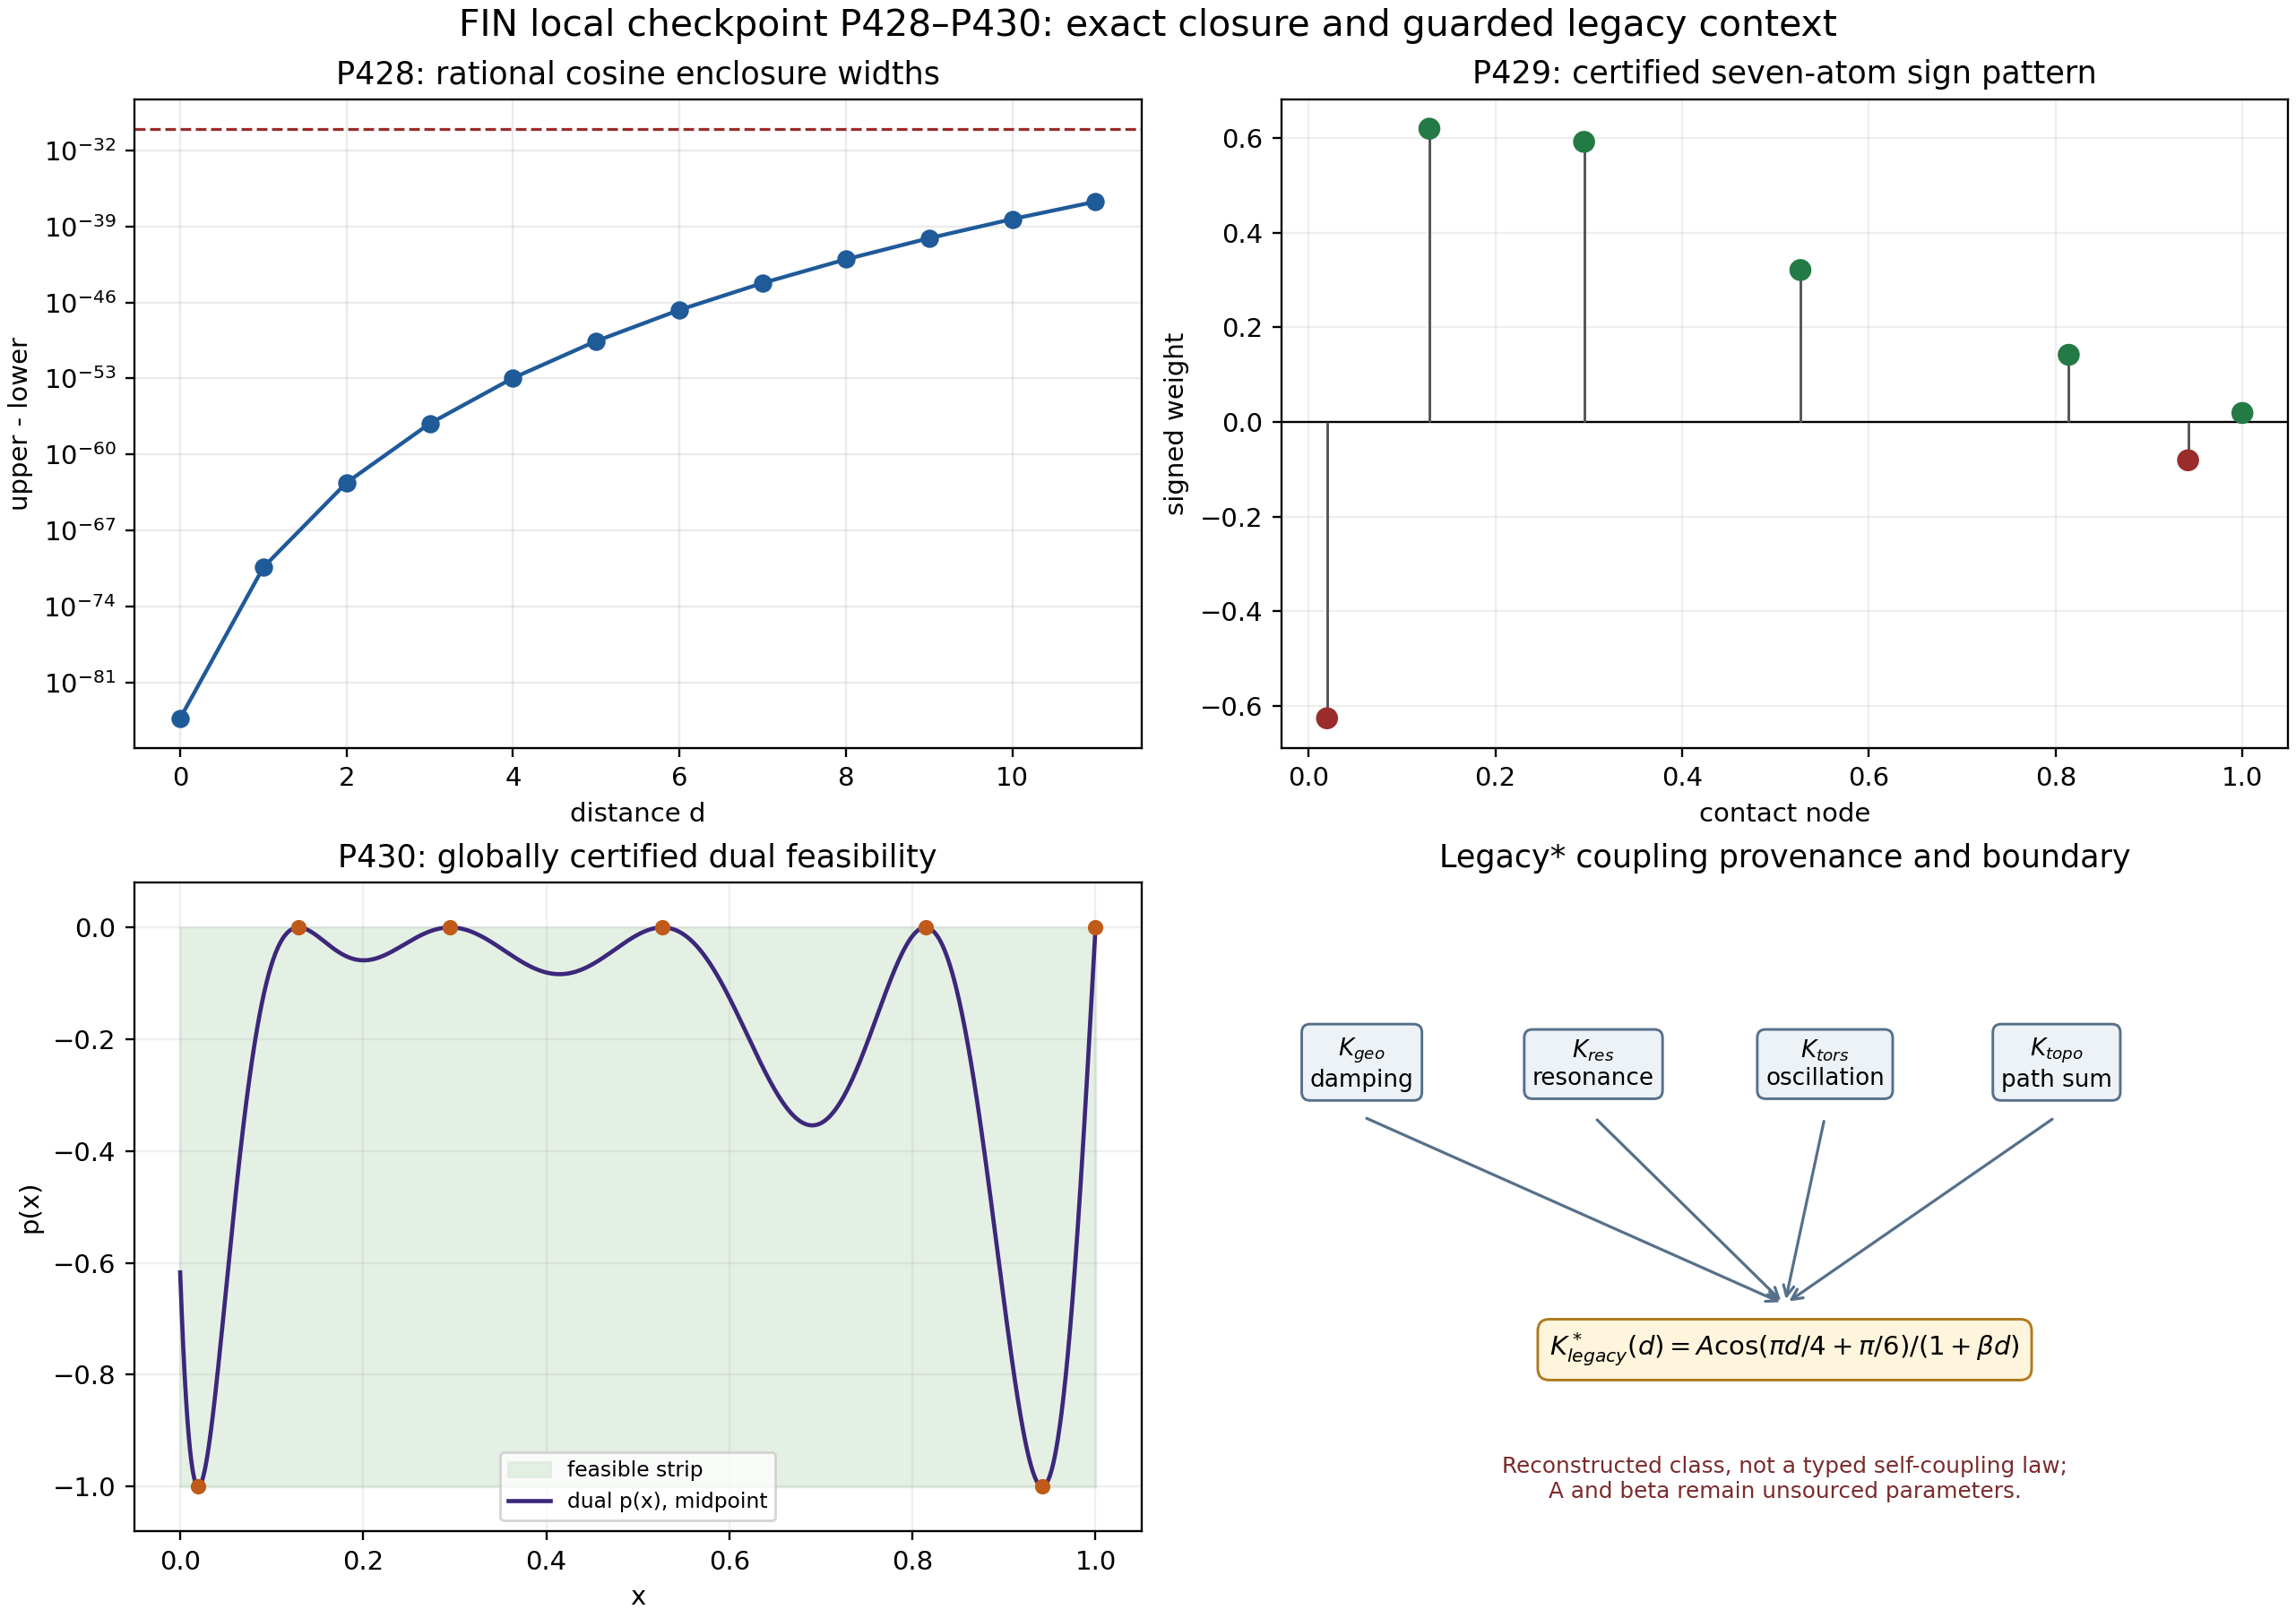
\includegraphics[width=\textwidth]{FIN_Programs_428_430_Figures/p428_p430_exact_closure_and_legacy_context.png}
\caption{Exact closure of P428--P430 and the guarded Legacy* coupling context.
The plotted polynomial is a midpoint visualization; the theorem comes from
the interval cells, not from the curve.}
\end{figure}

\section{Newly constructed typed objects}

\subsection{O155: Rational-Cut Cosine Provider Interface}

\begin{longtable}{p{0.24\textwidth}p{0.68\textwidth}}
\toprule
Field & Definition/audit\\\midrule
Domain/codomain & $\mathbb Q\to\operatorname{CutValue}$\\
Definition & Rational lower/upper predicates with compatibility\\
Required premise & Standard alternating-series cosine provider\\
Transformation law & Rational phase maps to its lower/upper cut\\
Generated theorem & All twelve P411 bounds from one provider\\
Necessity/removal & Reverting to \texttt{Rat -> Rat} reintroduces the type error\\
Kernel relation & Strict moment phases only; no legacy substitution\\
Selector dependence & None; no orientation is selected\\
Dimensional status & Dimensionless\\
Operational meaning & Formal trust boundary, not apparatus\\
Failure mode & Provider absent or used outside its domain\\
Confidence & \status{Proven interface/reduction; provider locally blocked}\\
\bottomrule
\end{longtable}

\subsection{O156: Exact-Rational Seven-Contact KKT Isolating Box}

\begin{longtable}{p{0.24\textwidth}p{0.68\textwidth}}
\toprule
Field & Definition/audit\\\midrule
Domain/codomain & Rational $X\subset\mathbb R^{25}$ and interval Krawczyk map\\
Definition & $\mathcal K=z_0-CF(z_0)+(I-CDF(X))(X-z_0)$\\
Premises & Moment enclosures, differentiable KKT map, rational preconditioner\\
Transformation law & Requires explicit transformation of variables and weighted norm\\
Generated theorem & One unique KKT zero in $X$\\
Necessity/removal & Without inclusion/contraction, O144 remains numerical evidence\\
Kernel relation & Built from strict moments; Legacy* is contextual, not input\\
Selector dependence & None\\
Dimensional status & Dimensionless\\
Operational meaning & Exact optimization certificate, not measurement\\
Failure mode & Inclusion or contraction reaches the box boundary\\
Confidence & \status{Computer-assisted proof}\\
\bottomrule
\end{longtable}

\subsection{O157: Contact-Aware Global Dual Certificate}

\begin{longtable}{p{0.24\textwidth}p{0.68\textwidth}}
\toprule
Field & Definition/audit\\\midrule
Domain/codomain & Interval coefficients/contact boxes to Boolean feasibility certificate\\
Definition & Curvature at contacts, monotonicity at $1$, Bernstein hulls on complement\\
Premises & O156 and exact contact equations\\
Transformation law & Affine interval maps preserve Bernstein hull bounds\\
Generated theorem & $-1\le p\le0$ on $[0,1]$\\
Necessity/removal & Without global cells, KKT stationarity is not dual feasibility\\
Kernel relation & Strict signed-moment dual only\\
Selector dependence & None\\
Dimensional status & Dimensionless\\
Operational meaning & Global mathematical witness, not observation\\
Failure mode & Any curvature, endpoint, or complement cell fails\\
Confidence & \status{Computer-assisted proof}\\
\bottomrule
\end{longtable}

No self-coupling object is named for the legacy diagram because its state map
and feedback law are absent.

\section{Falsification attempts and failed approaches}

\subsection{Type attack}
The P411 \texttt{Rat -> Rat} abstraction was tested against ordinary cosine
and rejected. The replacement represents irrational values by rational cuts
without pretending the values are rational.

\subsection{Conditioning attack}
The KKT Jacobian is extremely ill-conditioned. Precision was escalated to 180
decimals, but residuals alone were explicitly rejected. Exact interval
inclusion and the $q<1$ contraction bound survived.

\subsection{Exact-inverse expression swell}
Direct inversion of the 100-decimal rational Jacobian produced excessive
fraction growth on the declared hardware. The run was terminated without a
scientific result. A fixed rounded rational preconditioner gives the same
Krawczyk theorem interface and completed in seconds; no floating error is
silently imported because the rounded matrix itself is used exactly.

\subsection{Global-grid attack}
A dense plot was not accepted as evidence. Direct wide-interval evaluation can
overestimate near active contacts, so P430 separates contact geometry from
noncontact Bernstein cells. All proof cells pass at depth zero.

\subsection{Legacy diagram attack}
The diagram was treated as a falsifiable source, not an authority. Its path
exponent and integer-node sequence fail exact algebra. Its cross-modulations
survive only as an ansatz-level self-coupling intuition.

\subsection{Alternative explanation}
The P429/P430 object is fully explained as an extremal solution of a finite
signed-moment problem. Its existence does not establish a particle, field,
thermodynamic entropy law, observer mechanism, or laboratory channel.

\section{Numerical and formal reproducibility}

Repeated complete runs produced byte-identical JSON and CSV outputs.

\begin{longtable}{p{0.29\textwidth}p{0.62\textwidth}}
\toprule
Component & Method\\\midrule
P428 side conditions & Exact Lean rational arithmetic and \texttt{native\_decide}\\
P428 reflection & Python \texttt{Fraction} alternating sums\\
P429 root location & 180-decimal \texttt{mpmath} Newton iteration\\
P429 moments & Exact fractions, cosine Taylor/Lagrange enclosure, exact fifth-root brackets\\
P429 preconditioner & 70-decimal rational rounding of 180-digit inverse\\
P429 inclusion & Exact \texttt{Fraction} interval Krawczyk map\\
P429 uniqueness & Exact weighted infinity contraction $q<1$\\
P430 contacts & Exact rational interval curvature/value bounds\\
P430 endpoint & Exact rational interval derivative/value bounds\\
P430 complement & Exact affine power-to-Bernstein transform\\
Regression & Eight new tests plus inherited suites\\
\bottomrule
\end{longtable}

The local formal boundary is explicit: no real-cosine formal library and no
Mathlib are present. No dependency was downloaded and no Internet service was
used.

\section{Kernel, selector, dimensional, and operational audits}

\subsection{Kernel split}
P428--P430 consume strict moments. Legacy* appears only in the provenance
audit. Neither kernel is substituted for the other. The completion still
lacks source-independent phase/frequency, nonlinear compression,
amplitude/damping, selector, and unit data. Physical-role transfer remains
downstream and blocked.

\subsection{Selector}
O155--O157 are orientation-neutral certificates. They do not distinguish the
two signs of the $\mathbb Z_{12}$ orientation torsor. QW-2191 remains open.
The inversion-even radial Legacy* kernel also cannot supply a non-premise
directed selector.

\subsection{Dimensions}
All phases, moments, nodes, weights, polynomial coefficients, and evolution
parameters here are dimensionless. No action, length, time, mass, or energy
unit is internally generated. A numerical scale is not a physical unit.

\subsection{Dual dynamics and observer boundary}
For a self-adjoint $A$,
\[
U_t=e^{-itA},\qquad P_t=e^{-tA}
\]
are two functions of one spectral measure. This explains mathematical
wave/heat duality but supplies no physical state, preparation, calibrated
clock, reference frame, environment, instrument, apparatus response,
measurement record, custody, or hold-out unblinding.

\subsection{Physical evidence}
No data in this checkpoint are laboratory data. References in the historical
diagram to measurements, Wilson loops, or accuracy percentages are internal
repository claims and are not admitted as physical evidence.

\section{Scientific interpretation after this checkpoint}

The batch materially strengthens the mathematical core:
\begin{enumerate}
\item the cosine trust interface is correctly typed;
\item the seven-contact system has certified local existence and uniqueness;
\item its dual is globally feasible;
\item the signed-moment optimum has a certified value enclosure;
\item Legacy* has explicit provenance and self-coupling boundaries.
\end{enumerate}

It does not change the physical status of FIN. The deepest surviving
interpretation is a finite spectral/operator and signed-moment framework with
exact functional calculus, optimization certificates, and operational
interfaces. An external typed extension by state, preparation, clock,
reference frame, environment, instrument, apparatus response, dimensional
standard, and independent record is still required before experimentally
testable physics can be claimed.

\section{Ranked next local programs}

The next checkpoint should contain the bounded batch P435, P436, and P440.
No external gate will be simulated as evidence.

\begin{longtable}{r p{0.12\textwidth}p{0.58\textwidth}r}
\toprule
Rank & Program & Decisive local output & Probability\\\midrule
1 & P436 & Rigorous certification of at least one positive O149 erasure-code gain cell & 0.82\\
2 & P440 & Detector- and finite-sample-aware optimal JSR estimator, or minimax obstruction & 0.70\\
3 & P435 & Genuine noisy-comb SDP primal/dual certificate on one nonideal cell, or local solver obstruction & 0.62\\
4 & P432 & Exactly one complete-Bernstein/subordination damping-source class & 0.58\\
5 & P442 & Representation-independence audit of O153 oriented record current & 0.57\\
6 & P433 & Interval cover of one nontrivial photonic chart & 0.54\\
7 & P431 & Formal Lindemann--Weierstrass provider; no suitable local library exists & 0.10\\
\bottomrule
\end{longtable}

The first action is a cheap dependency and invariant audit. An expensive SDP
or minimax calculation begins only after its exact proposition and local
solver path are known.

\section{Artifact inventory}

\begin{itemize}
\item \path{FIN_Local_Research_Checkpoint_P428_P430_EN.md}
\item \path{FIN_Local_Research_Checkpoint_P428_P430_EN.tex}
\item \path{FIN_Local_Research_Checkpoint_P428_P430_EN.pdf}
\item \path{FIN_Current_Local_Research_Report_EN.pdf}
\item \path{RELEASE_10_36_PROGRAMS_428_430.md}
\item \path{FIN_Programs_428_430_Results.json}
\item \path{FIN_Programs_428_430_Summary.csv}
\item \path{FIN_Programs_428_430_P428_Cosine.csv}
\item \path{FIN_Programs_428_430_P429_Krawczyk.csv}
\item \path{FIN_Programs_428_430_P430_Global_Dual.csv}
\item \path{FIN_Programs_428_430_LegacyStar_Coupling_Audit.csv}
\item \path{FIN_Programs_428_430_P428_Cosine_Reduction.lean}
\item \path{FIN_Programs_428_430_Figures/p428_p430_exact_closure_and_legacy_context.png}
\item \path{fin_programs_428_430.py}
\item \path{test_fin_programs_428_430.py}
\item \path{FIN_PROGRAMS_428_430_RELEASE_MANIFEST.sha256}
\item \path{FIN_GOAL_STATE.md} and the checkpoint guardrail in \path{AGENTS.md}
\end{itemize}

\section{Restart instructions}

From the repository root:
\begin{verbatim}
MPLCONFIGDIR=/tmp/fin-mpl-cache python3 fin_programs_428_430.py
.elan/toolchains/leanprover--lean4---v4.28.0/bin/lean \
  FIN_Programs_428_430_P428_Cosine_Reduction.lean
MPLCONFIGDIR=/tmp/fin-mpl-cache python3 -m unittest -v \
  test_fin_programs_428_430.py
lualatex -interaction=nonstopmode -halt-on-error \
  FIN_Local_Research_Checkpoint_P428_P430_EN.tex
lualatex -interaction=nonstopmode -halt-on-error \
  FIN_Local_Research_Checkpoint_P428_P430_EN.tex
sha256sum -c FIN_PROGRAMS_428_430_RELEASE_MANIFEST.sha256
\end{verbatim}

Then inspect the state map and begin only the bounded P435/P436/P440 batch.
Preserve the local-only rule, kernel split, QW-2191 boundary, dimensional
boundary, and external-evidence gates.

\section{Conclusion}

O144 survives its decisive falsification tests. It is no longer merely a
floating-point pattern: inside a declared rational box it has exact existence,
local uniqueness, certified signs and ordering, and a globally feasible dual
polynomial. The resulting value is a rigorous computer-assisted theorem for
the declared dimensionless signed-moment problem.

The same rigor rejects overinterpretation. The reconstructed Legacy* kernel is
a legitimate intermediate historical mathematical class, but its diagram
provides neither typed self-coupling dynamics nor a source theorem for its free
parameters. The strict/legacy bridge, selector, dimensions, operational
apparatus, and empirical physics remain separate unsolved interfaces.

\end{document}
